%\documentclass[a4paper,UKenglish]{lipics-v2016}
%This is a template for producing LIPIcs articles. 
%See lipics-manual.pdf for further information.
%for A4 paper format use option "a4paper", for US-letter use option "letterpaper"
%for british hyphenation rules use option "UKenglish", for american hyphenation rules use option "USenglish"
% for section-numbered lemmas etc., use "numberwithinsect"
 

% Author macros::begin %%%%%%%%%%%%%%%%%%%%%%%%%%%%%%%%%%%%%%%%%%%%%%%%
%\title{\system: A Succinct Colored de Bruijn Graph Representation}
%\titlerunning{\system} %optional, in case that the title is too long; the running title should fit into the top page column

%% Please provide for each author the \author and \affil macro, even when authors have the same affiliation, i.e. for each author there needs to be the  \author and \affil macros
%\author{Fatemeh Almodaresi}
%\author{Prashant Pandey}
%\author{Michael A. Bender}
%\author{Rob Johnson}
%\author{Rob Patro}
%\affil{Stony Brook University, Stony Brook, NY USA\\
%  \texttt{\{falmodaresit,ppandey,rob.patro\}@cs.stonybrook.edu}}
%\authorrunning{Almodaresi et al.} %mandatory. First: Use abbreviated first/middle names. Second (only in severe cases): Use first author plus 'et. al.'

%\Copyright{Fatemeh Almodaresi,Prashant Pandey, Rob Patro}%mandatory, please use full first names. LIPIcs license is "CC-BY";  http://creativecommons.org/licenses/by/3.0/

%\subjclass{``E.1 DATA STRUCTURES'', ``E.2 DATA STORAGE REPRESENTATIONS'', ``E.4 CODING AND INFORMATION THEORY''}% mandatory: Please choose ACM 1998 classifications from http://www.acm.org/about/class/ccs98-html . E.g., cite as "F.1.1 Models of Computation". 
%\keywords{de Bruijn graph, succinct data structures, rank and select operation, colored de Bruijn graph}% mandatory: Please provide 1-5 keywords
% Author macros::end %%%%%%%%%%%%%%%%%%%%%%%%%%%%%%%%%%%%%%%%%%%%%%%%%

%Editor-only macros:: begin (do not touch as author)%%%%%%%%%%%%%%%%%%%%%%%%%%%%%%%%%%
%\EventEditors{}
%\EventNoEds{2}
%\EventLongTitle{}
%\EventShortTitle{}
%\EventAcronym{}
%\EventYear{2017}
%\EventDate{}
%\EventLocation{}
%\EventLogo{}
%\SeriesVolume{}
%\ArticleNo{}
% Editor-only macros::end %%%%%%%%%%%%%%%%%%%%%%%%%%%%%%%%%%%%%%%%%%%%%%%

%\begin{document}
\chapter{\system: A Succinct Colored de Bruijn Graph Representation\protect\footnote{A joint work with Prashant Pandey accepted in WABI2017}}
\label{sec:rainbowfish}
%\maketitle

\section{Abstract}
%
  The \cdbg --- a variant of the \dbg which associates each edge (i.e., \kmer)
  with some set of colors --- is an increasingly important combinatorial
  structure in computational biology. Iqbal \etal demonstrated the utility of
  this structure for representing and assembling a collection (population) of
  genomes, and showed how it can be used to accurately detect genetic variants.
  Muggli et al. introduced \vari, a representation of the \cdbg that adopts the
  \boss representation for the \dbg topology and achieves considerable savings
  in space over \texttt{Cortex}, albeit with some sacrifice in speed.  The
  memory-efficient representation of \vari allows the \cdbg to be constructed and
  analyzed for large datasets, beyond what is possible with \texttt{Cortex}.

In this paper, we introduce \system, a succinct representation of the color
information of the \cdbg that reduces the space usage even further. Our
representation also uses \boss to represent the \dbg, but decomposes the color
sets based on an equivalence relation and exploits the inherent skewness in the
distribution of these color sets. The \system representation is compressed based
on the $0$th-order entropy of the color sets, which can lead to a significant
reduction in the space required to store the relevant information for each edge. In practice,
\system achieves up to a $20\times$ improvement in space over \vari. \system is
written in \texttt{C++11} and is available at
\url{https://github.com/COMBINE-lab/rainbowfish}.
%


\section{~Introduction and Related Work}

This paper proposes a new representation of the \cdbg. The \cdbg is a variant of
the \dbg where each edge (i.e., \kmer) is associated with some set of colors.
Here, each color is used to encode the source of the corresponding \kmers (e.g.,
different source genomes, transcriptomes, sequenced samples, etc.). From this
perspective, it is a flexible and powerful combinatorial structure for
representing a collection of sequences while maintaining the identity of each.
This structure gained popularity in the work of Iqbal
\etal~\cite{Iqbal2012Novo}, which demonstrated the utility of the \cdbg for
representing and assembling a collection (population) of genomes, and for
detecting both simple and complex genetic variants with high accuracy. Analysis
of the \cdbg exhibits particular promise for analyzing complex population-level
variation, since topological structures (e.g., bubbles) can be associated with
variation in the underlying sub-populations. The representation adopted by
Iqbal, as implemented in the tool \texttt{Cortex}, is optimized for speed, and
so requires a considerable amount of memory to represent both the topology of
the \dbg and the colors associated with each edge.

The memory usage of the \cdbg representation adopted in \texttt{Cortex}
precludes this approach from being adopted when the underlying genomes and color
sets become too large. In order to overcome such limitations, Muggli et
al.~\cite{MuggliBoNo17} introduced the \vari representation of the \cdbg. This
approach sacrifices some of the speed of the \cortex representation for a
considerable reduction in the required space. \vari achieves this space savings
in two ways.  First, rather than using a hash-table-based representation of the
\dbg topology, it adopts the highly-efficient \boss representation. The
\boss~\cite{BoweOn12} representation (named based on the initials of the
authors) makes use of the FM index~\cite{FerraginaMa00} to encode the topology
of the \dbg. \boss uses $4N + o(N)$ bits to represent a \dbg with $N$ edges
(empirically, this often works out to be as few as 4-6 bits per edge).

\vari couples the \boss representation of the \dbg topology with a compressed
representation of the color information. By its nature, \boss assigns to every
\dbg edge a distinct rank in the range $[0,N)$. So, \vari represents the color
  information as a $N \times C$ bit matrix where $C$ is the number of input colors.
  Conceptually, each of the $N$ rows of this matrix is simply a bit vector that
  encodes which of the $C$ colors label the corresponding edge. To reduce the
  space required to store this color information, \vari concatenates these rows
  into a single vector over $N \times C$ coordinates and stores them in an
  Elias-Fano~\cite{Elias74, Fano71} encoded bit vector, allowing for a
  (sometimes substantial) reduction in the size while still enabling efficient
  point queries (i.e., is a particular edge labeled with a given color?).
  Muggli et al.~\cite{MuggliBoNo17} demonstrate that the \vari representation
  can be built on data sets consisting of large numbers of \kmers, large input
  color sets, or both.  Specifically, the space efficiency of \vari makes it
  possible to build and query the \cdbg on datasets that are orders of magnitude
  larger than what is possible with \cortex.  This is an exciting development
  that opens up this methodology for increasingly large-scale analysis.

  Though \vari achieves a substantial improvement in space over \cortex, there
  is still a considerable amount of redundancy present in its representation.
  Both of these systems represent the color set corresponding to each \kmer
  independently of other \kmers. Hence a considerable amount of redundant
  information can be present when the color set for each \kmer is represented
  independently. In fact, some existing colored de Bruijn Graph representations,
  like the Bloom Filter Trie~\cite{holley2016bloom} exploit this redundancy to
  compress shared color information, and share certain ideas and motivation with
  the representation proposed in this paper. However, many of the possible
  subsets of colors do not occur in practice, and there is an inherent (often
  extreme) skewness in the distribution of the color sets that do appear. It
  becomes even more important to exploit this skewness for large metagenomic
  datasets because the space usage of \vari for these datasets can become
  impractical.

  In this paper, we introduce a succinct representation, called \system, of the
  color sets associated to each edge in the \dbg. We also adopt the \boss
  representation of the \dbg topology, and focus, specifically, on how to
  concisely represent the color information. \system's \cdbg representation is
  entropy compressed and exploits the high skewness present in the distribution
  of color sets. By exploiting a more efficient decomposition of the set of
  present colors (i.e., in terms of equivalence classes), we achieve a
  considerable reduction over the space required by \vari (up to $20\times$
  depending on the dataset), while still retaining efficient (i.e., constant
  time) queries.

%In \system, we construct the color class representation from a color list from
%\vari~\cite{MuggliBoNo17} which in turn uses an efficient representation of
%the \dbg that they call it \boss~\cite{BoweOn12} based on the initials of the
%authors. This representation of \dbg is a generalization of FM indexes that
%can theoretically store a \dbg with m edges in $4m + o(m)$ bits and
%empirically stores \fatemeh{less than 6 bits per \kmer?}. In \boss
%representation we have a CD-lexicographical ordering of \kmers and the support
%for two operations of rank(k) and select(i) over this ordered set. rank(k)
%returns the number of elements before $\kmer_k$ and select(i) returns the
%exact value of \kmer that has $rank=i$. Both \vari and \system consider \kmers
%to be in the same order as returned by rank operation on \boss representation
%of \dbg. \system uses rank-and-select operation to map a \kmer to its color
%class. In the following section we briefly describe the rank and select
%operations. 

\section{~Background and definitions}

\system is a succinct representation of the color information, and uses rank and
select operations to lookup the color class corresponding to \kmers in the \dbg.
Here, we briefly recapitulate the definition of a succinct data structure and the
rank and select operations.

A \defn{succinct data structure} consumes an amount of space that is close to
the information-theoretic optimum. More precisely, if $Z$ denotes the
information-theoretic optimal space usage for a given data structure, then a succinct
data structure uses $Z + o(Z)$ space~\cite{Jacobson89}.

%\rp{this sub-sections seems redundant with the description above}
%\subsection{~\vari 's representation} In \vari the color information is
%stored, conceptually, a an subset from a set of $C$ colors for each of $N$
%\kmers are represented in a color matrix of size $N*C$ bits. If a bit in cell
%$(i, j)$ is set it means \kmer with rank $i$ has color $j$ (i.e. appears in
%$j^{th}$ sample). \vari compresses this uncompressed color matrix using either
%\rrr\cite{} or Elias-Fano\cite{} representation and achieves practical
%compression, but still in worse case scenario the color matrix storage is
%order of $N*C$.

\defn{rank} and \defn{select}~\cite{Jacobson89} are operations that are commonly
used for navigating within succinct data structures. For a bit vector
$B[0,\ldots,n-1]$, \rank$(j)$ returns the number of $1$s in the prefix
$B[0,\ldots,j]$ of $B$. \select$(r)$ returns the position of the $r$th $1$, that
is, the smallest index $j$ such that \rank$(j)=r$. For example, for the 12-bit
vector $B[0,\ldots,11]=$\texttt{100101001010}, \rank$(5)=3$, because there are
three bits set to one in the 6-bit prefix $B[0,\ldots,5]$ of $B$, and
\select$(4)=8$, because $B[8]$ is the fourth $1$ in the bit vector.

\section{~Method}
\label{method}

\begin{figure}[t]
  \centering
  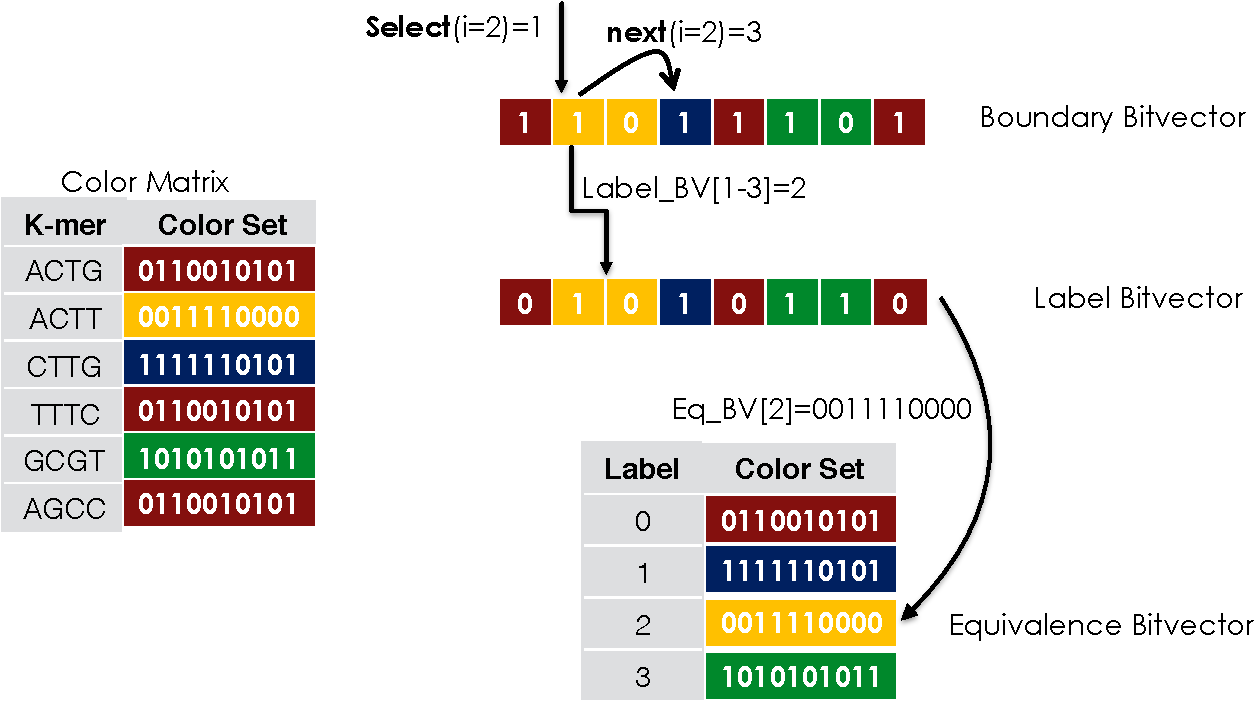
\includegraphics[width=\textwidth]{figs/cdbg-cropped}
  % \resizebox{0.80\linewidth}{!}{
  %   \ifpdf
  %     \input{cdbg-rep.pdf_tex}
  %   \else
  %     \input{cdbg-rep.eps_tex}
  %   \fi
  %   }
  \caption{
    The representation of color information in \system. The ``Color Matrix'' at
    the top represents $6$ distinct $4$-mers, each assigned a color set. $3$ of
    these $4$-mers (ACTG, TTTC, AGCC) have the same color class, labeled $0$,
    and the other $3$ (CTTG, ACTT, and GCGT) each have color classes labeled
    $1$, $10$, and $11$ respectively. To retrieve the color set for a \kmer, we
    first perform select on the boundary bit vector (BBV) using rank $r$ of the
    corresponding edge (\kmer). This returns the label's starting position, $i$.
    We then look for the next set bit BBV to find the label's ending position,
    $j$. Then, we fetch the label at indices $i$ to $j$ in label bit vector
    (LBV). Finally, we lookup the label $l$ in the equivalence class table (ECT)
    and return the color class corresponding to the label. A detailed
    explanation of the data structure and its construction is given in
    \Cref{design}.
  }
    \label{fig:cdbg-rep}
\end{figure}

In this section we first describe the design of \system. We then analyze the
space usage and provide a lower bound for the representation of sets of colors given
a ranking of \dbg edges. Finally, we discuss the \system implementation.

\subsection{~Design}
\label{design}

\system's compact representation of color information is based on two particular
observations. First, it is often the case that many of the \kmers in a \cdbg
share the same set of colors. More formally, we define an equivalence relation
$\sim$ over the set of \kmers in the \dbg. Let $\cfun{\cdot}$ denote the
function that maps each \kmer to its corresponding set of colors. We say that
two \kmers are color-equivalent (i.e., $k_1 \sim k_2$) if and only if
$\cfun{k_1} = \cfun{k_2}$. We will refer to the set of colors shared by the
\kmers related by $\sim$ as a \defn{color class}. If $C$, the number of input
colors, is large, it is often the case that the number of distinct color classes
is far less than the number of possible color classes (which is bounded above by
$\min(N,2^C)$).

Second, it is often the case that the frequency distribution of color classes
is far from uniform.  Hence, it will often be useful to record a frequently
occurring color class using a short description (i.e., a small number of bits)
while reserving larger descriptions for less frequent color classes.

%Put another way, both of these observations can be summarized in
%that we expect $H(X_c)$---the entropy of the color class---to be low (i.e., the
%expected value of the information available in each color class is low or
%order-$0$ entropy).

The design of \system is motivated by the above observations. Instead of storing
the color set for each \kmer separately, \system stores each distinct color
class only once and assigns to each distinct class a label (which, practically,
is much smaller than the unary encoding of the color class itself).
%
%\fatemeh{Furthermore, by replacing the fixed-length label with a variable-length
%one \system leverages the skewness property of distribution of \kmers across
%distinct color sets to save even more space.}
%
%starting from label 0 with 1 bit length. 
%
It then stores, for each \kmer, the label of the color class to which it
belongs. 
%
%Considering the skewed distribution of color class frequencies, this data
%structure can practically be much more efficient compared to the unary encoding
%of the color sets for each \kmer.

The approach we use to assign variable-length labels to color classes is similar
in spirit to the construction of a Huffman code, where the message is a string
of color class symbols. However, we do not build a prefix code, and instead opt
to store an additional bit vector to allow the efficient selection of an
arbitrary label from the list. We generate the labels according to the following
procedure. We first sort, in descending order, all the color classes based on
their frequency (i.e., the number of \kmers in this color equivalence class). We
then assign labels to each color class starting from the class with the largest
cardinality, so that the color class represented by the most frequent label will
have the shortest label length etc.

%The approach we use to assign variable-length labels to color classes is
%similar in spirit to the construction of a Huffman code, where the message is a
%string of distinct color sets (each representing symbol of a color class) and
%frequency of each symbol is frequency of each color class or in other words
%number of distinct \kmers observed with that color set. However, we do not
%build a prefix code, and instead opt to store an additional bit vector to allow
%the efficient selection of an arbitrary label from the list. We generate the
%labels according to the following procedure. We first sort, in descending
%order, all the color classes based on their frequency (i.e., the number of
%\kmers that display this color class). We then assign consecutive numbers as
%labels to each color class starting from the color class displayed by the most
%\kmers, so that the color class appearing as the most frequent label will have
%the shortest label length (which is 1 bit) etc.

The color class representation in \system has three components. \system stores
the mappings between labels and color classes in an \defn{equivalence class
  table (ECT)}. As labels are assigned sequentially, this is simply an array of
bit vectors encoding the corresponding color sets. Apart from the equivalence
class table, \system maintains two bit vectors, a \defn{boundary bit vector
  (BBV)} and a \defn{label bit vector(LBV)}.

All color classes are stored in the equivalence class table (with their
corresponding labels implicitly being their position). However, we now need to
store a mapping from \kmers to the variable-length labels. \system stores
variable-length labels corresponding to each \kmer in the label bit vector. The
labels are stored in the order in which \kmers are stored in the \dbg
representation. Specifically, the \kmers are stored in the rank order induced by
\boss. However, since these labels are variable-length, we can not directly read
the label corresponding to the \kmer of a specific rank, since we do not know
where such a label begins or how long it is.

To address this, \system maintains another bit vector --- the boundary bit
vector (BBV) --- to mark the boundary of each variable-length label in LBV. The
BBV is the same size as the LBV and has a bit set
to 1 at each index where a new label starts in the LBV. Thus, the starting
position for the label corresponding to the $r$th \kmer can be obtained by
issuing a \select{(r)} query on BBV, and the length of this label can be
obtained by simply scanning BBV until we encounter the next set bit.

\Cref{fig:cdbg-rep} shows how the color classes are represented in \system. To
perform a query for the color class corresponding to a \kmer in the \cdbg, we
first get the rank $r$ of the \kmer in the \dbg. We then perform a select
operation using $r$ on BBV. The result of the select operation $i$ is the start
index of the label of the color class in LBV to which the \kmer belongs.
%
To find the length of the label we determine the index $i'$ of the next bit set
in BBV using the \textsc{tzcnt} instruction.
%
\textsc{tzcnt} returns the number of trailing zeros in its argument. If $B$ is a
12-bit vector such that $B[0,11]=$\texttt{110010100000} then
$\textsc{tzcnt}(B)=5$.
%
%another select operation \fatemeh{we don't do that anymore} using $r+1$ to find
%the start of the next label. The difference between the start of the next label
%$i'$ and $i$ is the length of the label in the label bit vector. 
%
Using $i$ and $i'$ we retrieve the label from LBV, and using
the label we lookup the corresponding color class in ECT.
%
We also note that, as we never have $> 2^{64}$ distinct \kmers in practice, and
number of distinct labels is at max equal to the number of distinct \kmers (when
each \kmer has a unique label), then we never have $> 2^{64}$ labels. Hence, we can
always represent a label using a single machine word. Consequently, we will
always reach the next set bit in the LBV after scanning at most a single machine
word when starting from current label. This ensures we need only issue a single
\textsc{tzcnt} instruction per label decoding call.


\subsection{~Space analysis}
\label{system-space-bound}

The color class representation in \system is entropy compressed, i.e.,
the space is bounded by the entropy ($H(X_c)$) of the color class distribution. 
For a dataset in which number of \kmers belonging to each distinct color class are
similar, the entropy of the color class distribution will be high. On the other
hand, if most of the \kmers in a dataset belong to a small number of distinct
color classes, the entropy of the color class distribution will be low.

\begin{lemma}
  The size of each color class label is bounded by $\log_2{M}$ bits, where
  $M$ is the total number of distinct color classes. For a dataset with $N$
  distinct \kmers coming from $C$ input samples (i.e., colors), we have that $M
  \leq \min(N,2^C)$.
  \label{label-size-bound}
\end{lemma}

%\prashant{I have changed the wording in theorem 1. I don't know if it's better or worse.}

\begin{theorem}
Given an ordering of edges (or \kmers) in a \dbg, the space needed by \system to
represent a set of colors attached to each edge is $\order{MC+N H(X_c)}$ bits,
where $M$ is the number of distinct color classes, $C$ is the number of colors,
$N$ is the number of distinct \kmers, and $H(X_c) = -\sum_{i=1}^{M} P(x_i)\log
P(x_i)$ is the entropy (i.e., order-$0$ or Shannon's entropy) over random
variable $X_c$, which distributed according to the frequency distribution of the
color classes.
%$H(X_c)$ is the entropy of the color class distribution. 
\label{space-bound} \end{theorem}

\begin{proof}
%
The space needed by \system can be analyzed as follows. There are three bit
vectors in \system, the equivalence class table, label bit vector, and boundary bit
vector. To store an equivalence class table containing $M$ distinct color
classes each having $C$ colors we need $MC$ bits. To store a label bit vector
(as stated in \Cref{label-size-bound}), for $N$ \kmers, where each label
corresponds to one of the $M$ distinct color classes, takes $N\log_2{M}$ bits.
However, as explained in \Cref{design}, in \system we assign (optimal) variable-length
labels based on the frequency of color classes. Therefore, the space needed to
store the label bit vector is dependent on the $0$th-order entropy of the color
class variable, $H(X_c)$, and the size of the label bit vector is upper bounded
by $N\log_2{M}$.  The boundary bit vector has the same number of bits as the
label bit vector. 
%
\end{proof}

%%
% This seems redundant
%%
%As explained in \Cref{space-bound}, the space required to represent the label
%bit vector in \system depends on the entropy of the color class distribution.
%For a uniformly-random distribution the space would be high compared to a skewed
%distribution. The boundary bit vector contains the same number of bits as the
%label bit vector.


\subsection{~Lower bound for color representation}

%\fatemeh{I think we need a few sentences here to say we divide the space bound
  %to equivalence table space and label/boundary bit vectors and explain we are
  %already succinct regarding storing the equivalence table with space bound of
  %$\order{MC}$. Then say we now prove why we are also succinct regarding
  %label/boundary bit vectors with practical space of $\order{NH(X_c)}$}

We now provide a lower bound to store a color class representation for a set of
edges in a \cdbg. In the color class representation, the equivalence class table
takes $MC$ bits to store $M$ bit vectors each having $C$ bits, which is
optimal. The other two bit vectors, the boundary and label bit vector, map \kmers
given an ordering in the \dbg to their corresponding color classes. The theorem
below gives the lower bound to store such a mapping.
 
\begin{theorem}
%
  The lower bound to represent a mapping from an ordered list of \kmers in a
  \dbg to a set of color classes is $\log_2{(M^{N-M} \cdot M!)}$ bits, where
  $M$ is the number of distinct color classes, $N$ is the number of edges, and
  for a dataset with $N$ distinct \kmers coming from $C$ input samples (i.e.,
  colors), we have that $M \leq \min(N,2^C)$.
%
\end{theorem}

\begin{proof}

We can analyze the lower bound using a counting argument. We count the number
of ways to map a set of $M$ distinct color classes to a set of $N$ edges. The
space required to store the color class representation should be less than or
equal to the space required to store these mappings.

Edges can be mapped to color classes using a surjective (onto) function. Thus,
we wish to count the total number of surjections from $M$ color classes to $N$
edges. Rather than counting this number exactly, we instead provide a lower bound.
First, we must ensure that each of the $M$ color classes maps to at least one
edge --- so, we select a set of $M$ edges and label each with a distinct color
class. There are $M!$ ways to assign $M$ color classes to a set of $M$ edges. We
will then allow the remaining $N-M$ edges to be colored in any possible manner.
We can assign $M$ colors to $N-M$ edges (the remaining number) in $M^{N-M}$
ways. Therefore, the total number of different mappings is bounded below by $M^{N-M}
\cdot M!$. To be able to represent each such mapping, and distinguish it from
the others, we need at least $\log_2{(M^{N-M} \cdot M!)}$ bits.
\end{proof}

The lower bound can be expanded using Sterling's approximation as
\[
(N-M)\log_2{M} + M\log_2{M} - 0.44M + O(\log_2{M}),
\]
which, ignoring the
additive term $\order{\log_2{M}}$, is greater or equal to $N\log_2{M} - 0.44M$. Given the range of
$M$ (i.e., $1 \leq M \leq N$), $N\log_2{M}$ always dominates the lower bound.

Now, we show that the space needed by \system to store the variable-length
labels assigned to color classes is equal to the lower bound. As explained in
\Cref{label-size-bound}, the upper bound to store any label is $\log_2{M}$ bits,
and for $N$ edges, it is given by $N\log_2{M}$ bits.  \system also stores a
boundary bit vector which has the same number of bits as the label bit vector.
Therefore, the space required to store the label mappings is strictly $\leq
2N\log_2{M}$. Note that the extra overhead to store the metadata to perform a
select operation in constant time on the boundary bit vector is bounded by
$o(N)$, where $N$ is the numbers of bits in the bit
vector~\cite{GonzalezGrMa05}.

However, \system's representation of color classes is entropy compressed (see
\Cref{design}) and the space required depends on the entropy of the color class
distribution. For a highly skewed distribution, the entropy is low and the space
required to store labels is much smaller than $N\log_2{M}$ bits. On the other
hand, when the distribution is near-uniform, i.e., the entropy is high, \system
makes all labels to be $\log_2{M}$ bits and dispenses with BBV. Therefore, the
space required by \system is always smaller than or equal to the lower bound.

%\fatemeh{Here we are proving ds <= O(Z) while for succinct we should prove ds
%= Z + o(Z). The first is the proof for compact. So one idea we discussed with
%Robp is to remove $\order{}$ from $\order{N\log_2{M} -/+ blabla}$ and consider
%it as $Z'$ which is itself a lower bound on Z ($Z' = Z + o(Z)$). Then we prove
%ds = $Z' + o(Z') = Z + o(Z) + o(Z + o(Z)) = Z + o(Z)$}


\subsection{~Implementation}

\tikzsetnextfilename{plant-eq-class-dist}
\begin{figure}[h]
\centering
\begin{tikzpicture}[scale=0.8]
  \begin{axis}[
    ybar,
    %x=2pt,
    %height=6cm,
    bar width=3pt,
    xtick=data,
    scaled ticks=false,
    ymode=log,
    ymin=0,
    ylabel={\#\kmers in each equivalence class},
    xlabel={Equivalence class labels},
    legend style={at={(1.05,0.63)}, anchor=north west},
    nodes near coords align={vertical},
  ]
    \pgfplotstableread{data/plant-eqDist-1pass}\loadedtable;

      \addplot[color=teal, fill=teal] table[x=x_0, y=y_0] {\loadedtable};
      \addplot[color=olive, fill=olive] table[x=x_0, y=y_1] {\loadedtable};
      %\addplot[color=teal, fill=teal] table[x=x_0, y=y_2] {\loadedtable};
      \legend{Color class dist. in $1$-pass,Color class dist. in $2$-pass}
    \end{axis}
\end{tikzpicture}
    \caption{
    Distribution of \kmer frequencies across equivalence class labels in \system
    after $1$-pass and $2$-pass algorithm on plant dataset
    \Cref{tab:datasets-info}. The $2$-pass algorithm assigns the smallest label
    to color class with maximum number of \kmers. The distribution in $2$-pass
    algorithm is monotonically decreasing. 
  }
      \label{fig:plant-eq-class-dist}
\end{figure}

\subparagraph{Considerations due to the underlying \dbg representation} We recall here that we make use of the BOSS representation of the underlying \dbg topology. To build the BOSS representation, \kmer counting is first performed using KMC2~\cite{Deorowicz15KMC}, canonicalizing \kmers during counting. Though the BOSS representation inserts both forward and reverse complement \kmers into the graph, it associates only a single color vector with this pair.  Moreover, BOSS creates ``dummy'' edges (real \kmers prepended or appended with \$) to allow encoding \kmers that appear near terminal nodes in the \dbg. In the \cdbg these dummy edges are assigned the empty color set. All of this information is encoded by both \vari and \system. However, as we discuss in more detail in~\Cref{sec:conclusion}, the \system representation can work with any \dbg representation that can assign distinct ranks to each \kmer in the \dbg. Thus, we would expect this encoding scheme to work well with, e.g., a \dbg representation based on minimum perfect hashing of the
\kmers~\cite{drezen2014gatb}.
%\fatemeh{We should note that as BOSS counts a \kmer and its reverse complement as two distinct \kmers, we also count them as two different \kmers.}

\subparagraph{Storing bit vectors.} In \system, we use bit vector implementations
from the SDSL library~\cite{sdsl} to store the three bit vectors from
\Cref{fig:cdbg-rep}. We use the $rrr\_vector$ implementation from SDSL to store
the equivalence class table and boundary bit vector, and the $bit\_vector$ implementation
from SDSL to store the label bit vector.

The $rrr\_vector$ of SDSL is an implementation of \rrr encoding~\cite{RamanRaRa02}. \rrr
encoding is an entropy compressed encoding and also supports constant time rank
and select operations on the compressed bit vector.  The space reduction depends
on the entropy of the bit vector. For high entropy bit vectors, the compression
is not noticeable and in fact ``negative'' in some cases because of the extra
metadata overhead to support rank and select operations.

The equivalence class table and boundary bit vector often have fairly low
entropy, and can be compressed efficiently using RRR encoding. However, the
label bit vector often has high entropy, and compressing it using \rrr encoding
is not effective. In our representation, the average order-$0$ entropy of the
label bit vector for four different datasets is $0.94$. This is a quite high,
and hence we did not see any reduction in the space using \rrr encoding.
However, for the other two bit vectors, the order-$0$ entropy is lower (e.g.,
for boundary bit vector the average entropy over same four datasets is $0.56$)
and, in practice, we achieve a considerable space reduction using RRR encoding.

\subparagraph{Construction.} We use a $2$-pass algorithm to construct the three bit vectors. In the first pass, we read the color matrix, compute the distinct color classes, and count the frequency of each class. Once we have the frequency information, we sort color
classes in descending order based on their frequency. We then assign labels to
color classes starting from zero. In the second pass, we read the uncompressed
color matrix again, and add the label of each \kmer to the label bit vector.
While building the label bit vector, we also build the boundary bit vector by
storing a $1$ at every index where a new label starts in the label bit vector.
The labels are stored in the same order as the \kmers in the \boss
representation.

To reduce the space required for the labeling even further, we implemented our label
encoding in the following way. Every time that the label size increases from $x$
bits to $x+1$ bits, we restart the counter of that label in label bit vector to
$0$. For example, we store $0$ and $1$ for labels $0$ and $1$ respectively,
then we store $00$, $01$, $10$ and $11$ for labels $2$, $3$, $4$ and $5$
respectively. For label value $6$ we again restart the counter to $0$ and store
$000$ to represent $6$ in the label bit vector, etc. Later, when we want to retrieve
the actual value of a label, we first recover the stored label $l'$ from the label
bit vector and then calculate the actual label $l$ using the equation $l = l'
+ 2^{d}-2$ where d is length of label $l$ in bits.

As explained in \Cref{system-space-bound}, the $2$-pass algorithm minimizes the
space used to represent color class labels by sorting the classes based on their
frequencies and assigning labels to color classes to minimize the length of the
resulting code path, similar to Huffman coding. However, one could also imagine
assigning labels to color classes as we see them in the order \kmers appear in
the \boss representation. This way, we can construct all three tables in a single
pass (i.e., a $1$-pass algorithm).

However, as shown in \Cref{fig:plant-eq-class-dist}, this $1$-pass algorithm can
end up assigning long labels to frequent \kmers, and hence produce poor (i.e.,
large) encodings. However, the $2$-pass algorithm always assigns labels
according to the corresponding frequency distribution of the color classes.
Sometimes, the $1$-pass algorithm does well, but we chose to adopt the $2$-pass algorithm
in \system. 

\section{~Evaluation}

\begin{table}
  \begin{center}
    \begin{tabular} {| l | c c c|}
    \hline
      Datasets & \# of edges & \# of colors (samples) & \# of distinct color classes \\
      \hline
      \ecoli 10 & 28,273,951 & 10 & 479\\
      \ecoli 1000 & 157,737,064 & 1000 & 2,669,157 \\
      \ecoli 5598 & 435,705,390 & 5598 & 7,000,715\\
      \ecoli 1000 (k=63) & 258,893,268 & 1000 & 2,530,253\\
      Plant & 2,520,140,426 & 4 & 16 \\
      Beef safety & 97,096,576,010* & 87 & 623,022,532\\
      Human transcriptome & 159,441,804* & 95,146 & 340,762\\
      \hline
      % &  e-coli 10 & e-coli 1000 & e-coli 5598 & Plant & Beef Safety \\
      %Num. of Edges &  & 157,737,064 & 435,705,390 & 2,279,614,458 & \\
      %Num. of Colors & 10 & 1000 & 5598 & 4 & 87 \\
    \end{tabular}
  \caption{
    The number of edges (include \kmers and dummy edges in the BOSS
    representation), samples and color classes for different datasets used in
    the experiments. $k = 32$ unless otherwise specified. \small
    *\# of edges excluding dummies.
}
\vspace{-2.5em}
  \label{tab:datasets-info}
\end{center}
\end{table}

\begin{table}
\begin{center}
\begin{tabular} {| l | c c| c c|}
\hline
Datasets & \multicolumn{2}{c|}{Construction Time (secs)} & \multicolumn{2}{c|}{Bubble Calling Time (secs)} \\
\cline{2-5}
& \vari & \system & \vari & \system \\
\hline
\ecoli 10 & 44 & 31 & 344 & 366\\
\ecoli 1000 & 340 & 270 & 2,610 & 2,356\\
\ecoli 5598 & 3,141 & 4,021 & 8,796 & 8,201\\
%\ecoli 1000 (k=63) & 323 & 257 & 3,971 & 7,546\\
\plant & 108 & 339 & 47,040 & 48,537\\
\beefsafety & 15,378 &  30,478 & NA & NA\\
Human transcriptome & 13,961 & 30,804 & NA & NA\\
\hline
\end{tabular}
\caption{
  Construction and bubble calling time for \system and \vari for different
  datasets. 
}
\vspace{-2.5em}
\label{tab:time}
\end{center}
\end{table}

In this section we evaluate \system, and compare it to \vari~\cite{Muggli17}, a
state-of-the-art \cdbg representation. We evaluate both systems in terms of
space and running time. We address the following questions about the performance
of \system: How does \system compare to \vari in terms of the space required to
represent color information?; How does \system compare to \vari in terms of the
construction time?; How does \system compare to \vari in terms of typical
queries (e.g., in bubble calling)? We are particularly concerned with ensuring
that \system produces small encodings of the color information and remains
practically efficient to query.

\subsection{~Experimental setup}

To answer the above questions, we perform two different benchmarks. First, we
evaluate the time taken to construct the color class representation. The
construction time is the time taken to construct the color class representation
from a list of color classes stored in the order of the edges in the \dbg (this
is the same input used by \vari). During construction, we adopt a two-pass
algorithm. In the first pass, we use a sparse hash-table to determine the distinct
color classes and the cardinality of each such class.

We note that the space taken in this first pass is within a small constant
factor of the final space required by the final ECT table itself, since we need
only store each color class once in the hash table (as a key), and store the
associated count (a machine word) as the value.  Thus, the memory required by
this first pass is almost always a small fraction of the total memory usage 
of the construction algorithm.

Given this information, we know exactly the number of bits that will be required
to store the label and boundary vectors. In the second pass, we fill in both the
label and boundary vectors and then save all three structures to file. As with
most succinct representations, the space required for our data structure in
memory and on disk is almost the same (as the two-pass algorithm allows us to
allocate only the space we need for our final representation). The construction
time recorded here does not include (for either \system or \vari) the time taken
to build the \dbg and color list corresponding to edges in the \dbg (since this
is the same for both methods).

We also report the space needed by both \system and \vari to store the color class
representation on disk. We do not include the space needed to represent the
actual \dbg in our space comparisons because both \system and \vari use \boss
to store the actual \dbg, and the \boss representation itself tends to take less
space than the color information.

Second, we evaluate the time taken to perform the bubble calling benchmark as
described in~\cite{MuggliBoNo17}, using both the \vari and \system
representations. Finding bubbles in a \cdbg enables one to detect regions in the
\dbg where different samples (i.e., colors) diverge from each other. As
originally suggested by Iqbal et al.~\cite{Iqbal2012Novo}, such algorithms can
form the basis for analyzing certain types of genetic variants in populations of
genomes. We note that we adopt the exact bubble calling algorithm implemented in
\vari, and the only variable being altered in our bubble-calling benchmark is
the data structure being used to determine the set of colors present for each
\kmer. Since \vari and \system are both built upon the \boss representation,
which is based on the edge-centric view of \dbg, they consider \kmers as edges
in the \dbg, meaning that each edge is associated with a \kmer, and its
corresponding rank and color set. Briefly, the bubble calling algorithm takes as
input a pair $c_1,c_2$ of colors and traverses edges in the \dbg to find bubbles
in which the edges in one sub-path are colored with $c_1$ and the edges in the
other sub-path are colored with $c_2$ (see~\cite{MuggliBoNo17} for further
details).

For all experiments in this paper, unless otherwise noted, we consider the \kmer
size to be $32$ to match the parameters adopted by Muggli et
al.~\cite{MuggliBoNo17}. We carry out these benchmarks on a number of datasets
as described in \cref{subsec:data}. The time reported for construction and
bubble calling are averaged over two runs, and the time is measured as the
wall-clock time using the \texttt{/usr/bin/time} executable. All experiments
were performed on an Intel(R) Xeon(R) CPU (E5-2699 v4 @2.20GHz with 44 cores and
56MB L3 cache) with 512GB RAM and a 4TB TOSHIBA MG03ACA4 ATA HDD running ubuntu
16.10, and were carried out using a single thread. We note that, while the
construction of the color set representation in \system (and \vari) are serial
operations, queries are trivially parallelizable, as each label can be queried
and decoded independently.

\subsection{~Data}
\label{subsec:data}

We run our benchmarks on the datasets mentioned in \Cref{tab:datasets-info}.
The first three datasets, 
%All three datasets 
\ecoli, \plant, and \beefsafety are slight variants of those used for
evaluation in \vari~\cite{MuggliBoNo17}. Each of these data sets exhibits
different characteristics in terms of the number of \kmers, the number of input
samples (i.e., colors) and the homogeneity of the underlying samples (i.e., how
different are the \dbg for each of the individual samples).
%
The first dataset consists of the assemblies of 5,598 different strains of
\ecoli obtained from GenBank~\cite{o2015reference}. Here, each ``color''
represents a specific \ecoli assembly. Since these assemblies are from
different strains of the same species, they exhibit a small degree of
heterogeneity. In other words, a large fraction of the union \dbg is expected
to occur in all samples.

To evaluate the scalability of \system when primarily changing the underlying
number of input colors, we have evaluated three variants of the \ecoli dataset.
These consist of a dataset containing only 10 different strains, another
containing 1,000 different strains and the final containing all 5,598 strains.
We also performed experiments with \kmer size to be $63$ for \ecoli 1000
dataset to evaluate the space usage for higher \kmer sizes.


%All these experiments are conducted on set of \kmers derived from
%the data with $k=32$. In addition to that, to evaluate the effect of k in for
%\kmers in the space required by \system we ran it \kmers with $k=63$ from
%\ecoli 1000.

%Using all \ecoli assembly samples we will have \kmers from 5,598 different
%colors. To evaluate the effect of varying number of colors on storage and
%performance of \system, we design three different experiments on \ecoli data
%running all steps of the process on the first 10, 1000, and then all 5,589
%\ecoli samples. 
The second dataset (i.e., \plant) consists of the genome assemblies of four
different plant species. Hence, this dataset contains only four colors, but has
more than $\approx2$ billion distinct \kmers. The plant species considered are,
\fnurl{\textit{A}. \textit{thaliana}
}{ftp://ftp.ensemblgenomes.org/pub/plants/release-34/fasta/arabidopsis_thaliana/dna/Arabidopsis_thaliana.TAIR10.dna.toplevel.fa.gz}~\cite{swarbreck2008arabidopsis},
\fnurl{Corn}{ftp://ftp.ncbi.nlm.nih.gov/genomes/all/GCF/000/005/005/GCF_000005005.1_B73_RefGen_v3/GCF_000005005.1_B73_RefGen_v3_genomic.fna.gz}~\cite{schnable2009b73},
\fnurl{Rice}{http://rice.plantbiology.msu.edu/pub/data/Eukaryotic_Projects/o_sativa/annotation_dbs/pseudomolecules/version_7.0/all.dir/all.con}~\cite{tanaka2008rice},
and
\fnurl{Tomato}{ftp://ftp.solgenomics.net/tomato_genome/assembly/build_2.50/SL2.50ch00.fa.tar.gz}~\cite{causse2013whole}.
%
These genomes exhibit considerable diversity and heterogeneity. Given the
diverse regions in the \cdbg, this dataset is a good candidate for the bubble
calling benchmark. Further, Muggli et al.~\cite{MuggliBoNo17} found that this
was the only of the three original datasets on which they were able to construct
the original \texttt{Cortex} representation of the \cdbg. They validated
\texttt{Cortex} produces the same bubble calls as \vari ~\cite{MuggliBoNo17}
(which, of course, produces the same bubble calls as \system).
%
For more detailed analysis of \texttt{Cortex}'s construction and processing time
and space on this dataset, please refer to~\cite{MuggliBoNo17}.
%
%among different samples that later will be critical for time evaluation in
%bubble finding process as there will be a lot of branching in \dBG and hence a
%lot of access queries for pair of \kmer and color on each branch. 
%

The third dataset, \beefsafety, is considerably different from the prior data.
Instead of the input samples consisting of assembled genomes, they consist of
87 metagenomic samples sequenced from cattle in the commercial process of beef
production~\cite{noyes2016resistome}. Hence, this dataset yields a considerably
larger and more complex \dbg since it is built upon many un-assembled (and
non-error-corrected) reads. Thus, the \dbg will encode portions of the relevant
metagenomes as well as the effects of sequencing errors. This dataset also has
many more \kmers than the others, $\approx97$ billion. It exhibits a large
degree of heterogeneity and an intermediate number of input colors (87).
%
%is a doubly huge dataset with total amount of 97,096,576,010 \kmers and
%considerable number of colors (87) and heterogeneity which provides a good
%practical example to evaluate time and space of \system compared to
%state-of-the-art colored \dBGs, \vari. 
%

In addition to the three datasets used in the \vari paper, we also consider
building the \cdbg on the \fnurl{human
transcriptome}{ftp://ftp.sanger.ac.uk/pub/gencode/Gencode_human/release_26/gencode.v26.pc_transcripts.fa.gz}
(Gencode v26 protein coding transcripts)~\cite{Harrow2012}. Here, we consider
each transcript as an individual sample (i.e., a distinct input color). This
data consists of $\approx95,000$ colors, but only $\approx159$ million \kmers.
Hence, this dataset will give an idea about how the representations
will perform when the number of colors becomes very large (though the number of
distinct color classes remains orders of magnitude smaller than the number of
\kmers). Further, we note that this dataset highlights some of the similarities
between the color class encoding adopted by \system and the \kmer-based
equivalence class decomposition adopted by certain transcript quantification
methods (e.g.~\cite{PatroSailfish:2014}).

%The fourth dataset illustrates another use case for \cdbg tools other than
%metagenomic analysis. This dataset is human transcriptome in which we consider
%each transcript as an individual sample, so that the \cdbg built upon this
%dataset has as many colors as transcripts.

%\footnote{ftp://ftp.ensemblgenomes.org/pub/plants/release-34/fasta/arabidopsis_thaliana/dna/Arabidopsis_thaliana.TAIR10.dna.toplevel.fa.gz}
%,
%\fnurl{Corn}{ftp://ftp.ncbi.nlm.nih.gov/genomes/all/GCF/000/005/005/GCF_000005005.1_B73_RefGen_v3/GCF_000005005.1_B73_RefGen_v3_genomic.fna.gz},
%Rice
%\footnote{http://rice.plantbiology.msu.edu/pub/data/Eukaryotic_Projects/o_sativa/annotation_dbs/pseudomolecules/version_7.0/all.dir/all.con}
%and Tomato \footnote{
%ftp://ftp.solgenomics.net/tomato_genome/assembly/build_2.50/SL2.50ch00.fa.tar.gz}

\subsection{~Performance}

\Cref{tab:time} shows the time taken by \system and \vari to construct the color
class representation for different datasets. \system uses a $2$-pass algorithm
to construct the color class representation, and hence the construction time is
dominated by the steps to read the color list file twice. For small datasets
like \ecoli $10$ and \ecoli $1,000$, the input file size is small and does not affect
the overall construction time compared to \vari. However, for large datasets
like \plant and \beefsafety, the time to read the color file twice dominates the
construction time and \system is $1.9\times$---$3\times$ slower. We note that
this time can be considerably reduced by avoiding the uncompressed color matrix
representation currently used upstream of \system and \vari, and integrating
determination and encoding of the color classes into the \dbg construction
directly. However, this is outside the scope of the current paper.

\paragraph*{~Space}\Cref{tab:space} shows the space usage of \system and \vari
for the different datasets we consider. Among these data, there are a range of
characteristics in terms of the number of \kmers, the number of colors, and the
complexity and heterogeneity of the \dbg. We find that, for all datasets,
\system requires less space to store the color information than \vari.  The
magnitude of the improvement depends on the number of distinct equivalence
classes and their distribution, but is as large as $\sim 20\times$.  We see the
same trend with higher values of \kmer sizes.

%\fatemeh{Even changing $k$ to higher value doesn't change the trend.}

In particular, \system's space usage is particularly impressive for datasets
with a large number of input colors but a relatively small number of distinct
\kmers. In this case, we usually find that the number of distinct color classes
is very small compared to the universe of possibilities, and so each label can
be encoded in much fewer than $C$ bits. However, the space \vari consumes
depends greatly on the sparsity of the color matrix. The color matrix itself
grows rapidly as the number of \kmers and colors increases, but \vari's
compression mechanism (Elias-Fano encoding) is very effective if the color
matrix is sparse (e.g., each \kmer is labeled with only a small subset of
colors). This is exactly the case for the Human transcriptome, where the color
matrix has an entropy of $\sim 0.0004$ (compared to \ecoli 5,598 and \ecoli
1,000 with entropies of $\sim 0.16$ and $\sim 0.34$ respectively). Thus, in the
\ecoli dataset, \vari can save space up to a factor of $\sim 5$ compared with
the uncompressed representation, while in the Human transcriptome it can save a
factor of $\sim 2,150$ because of the low entropy of the color matrix. \system
does well in all experiments, even when the number of input colors is small
(e.g., in the \plant dataset). \system achieves the most impressive compression
when the color class distribution has low entropy and the number of color classes
is small relative to the upper bound.
In such cases, the entropy compressed representation of \system is able to
represent a large fraction of all labels using a very small number of bits.
%\fatemeh{
%while because of high entropy in color matrix, \vari's space increases as a result of negative compression. 
% --> This low entropy in color class distribution and high entropy in color matrix might be a little bit confusing but really interesting to talk about.} 


\begin{table}
\begin{center}
\begin{tabular} {| l | c c c|}
\hline
Datasets & 
uncompressed color matrix & \vari & \system \\
\hline
\ecoli 10 & 34 & 58 & 20 \\
\ecoli 1000 & 18,804 & 8,848 & 475 \\
\ecoli 5598 & 290,761 & 58,718 & 2,938 \\
\ecoli 1000 (k=63) & 185,669 & 8,872 & 637\\
\plant & 1,202 & 1,603 & 497 \\
\beefsafety & 1,007,009 & 210,998 & 144,564 \\
Human transcriptome & 1,808,435 & 841 & 817 \\
\hline
\end{tabular}
\caption{
  The space required by \system and \vari to store the color class
  representation for different datasets. The first column shows space required for the uncompressed color matrix ($N \times C$ bits).
  All space is reported in MB. $k = 32$ unless otherwise specified.
}
\vspace{-3.5em}
\label{tab:space}
\end{center}
\end{table}

%Based on the design of our data structure we would expect to see an order of
%magnitude improvement in storage as number of colors increase. We expect to do
%as well as \vari in case of 10 samples of \ecoli as a small dataset with few
%colors and do much better regarding space in case of considering all 5,598
%samples. table \ref{tb:space} shows changes of storage while changing number
%of colors. As shown in table \cref{tb:space} \system improves space when
%number of colors increase from taking 16 times less space in \ecoli with 1000
%samples to 26 times in full \ecoli dataset compared to \vari. 

%Another interesting result is the huge amount of space improvement we see in
%\plant dataset although it has just four colors which implies that \system not
%only works better in terms of increasing number of colors but also when we have
%a huge amount of \kmers. While in \vari, they keep four bits per each \kmer in
%\plant dataset (one bit for each color and hence four bits for four colors),
%but still replacing that with two bits for the first two most frequent color
%sets in \system can still save a lot of space when we have a considerable
%amount of \kmers even with the overload of saving equivalence table.

\paragraph*{~Bubble calling} \Cref{tab:time} shows the time taken by \system and \vari to perform the bubble
calling benchmark on different datasets. We run the bubble calling benchmark on
the \ecoli and \plant datasets (as in the \vari paper). We note that the current
bubble calling algorithm is too slow to run on the Beef safety data set (the
time in~\cite{MuggliBoNo17} was estimated at $>3,000$ hours). It is possible,
however, that optimizations to the underlying algorithm might lift this
restriction. We also did not perform bubble calling on the human transcriptome
dataset as here, we were unable, given the resources on our server, to even run
the \dbg construction to completion. Specifically, due to the large amount of
external memory that \vari uses to build the uncompressed color matrix and the
\dbg on these larger (either in terms of the number of \kmers, the number of
colors, or both) datasets (on order of Terabytes), we exhausted the available
disk space. For these datasets, to approximate the relevant sizes and
construction times, we produced a uncompressed color matrix that lists the
colors for each \kmer and its reverse complement, and we use this to build both
the \vari and \system color representations. While very similar to the full color
matrix that \vari would produce, this file is slightly different in that it does
not include entries for dummy edges (a detail of the \boss representation), and
the order of the color matrix rows can be different from what will appear in the
\boss representation. However, we still believe these numbers, provided in
\Cref{tab:datasets-info}, give a reasonable approximation of how the respective
methods would perform were we able to construct the \dbg completely.

For bubble calling, both representations require a very similar amount of time.
This is likely due, in part, to the fact that navigating the \boss
representation of the \dbg may be the performance bottleneck in the bubble
calling algorithm. Thus, both \vari and \system provide sufficiently fast access
to the color sets for each edge that they do not represent bottlenecks in this
regard.

\section{~Conclusion and Future Work}
\label{sec:conclusion}

In this paper, we propose an entropy-compressed, succinct data structure to
store the color information of a \cdbg. To represent the topology of the \dbg
itself, we adopt the \boss~\cite{BoweOn12} representation. However, we note
that, for our representation of the color sets, we only require that the
underlying \dbg representation is able to associate a unique rank between $0$
and $N-1$ with each edge. Hence, it is possible to use the \system
representation with other representations of the \dbg topology (e.g., those
based on minimal perfect hashing).

We demonstrate that the inherent skewness in the distribution of color classes
can be exploited to reduce the size of the color information. This allows
\system to represent the \cdbg, even for large datasets with many colors, in a
reasonably small space. In fact, for representing the color information itself,
we show that \system is succinct, and hence requires only $Z + o(z)$ bits where
$Z$ is the number of bits required by an information-theoretically optimal
representation.
%
Moreover, it may be possible for the color information stored in the equivalence
class table to be further compressed to reduce the space. For example, one could
imagine an encoding of color sets that takes advantage of their shared subsets,
e.g., storing the shared prefixes of membership vectors only once.
%
%It's also likely that reordering \kmers would reduce the entropy of the label
%vector and result in higher compression ratio. For example, \kmers appearing
%nearby in the \dbg have a higher probability of having the same color class.
%Reordering \kmers based on the \dbg traversal order can bring \kmers with same
%equivalence classes together and thereby increasing the skewness in the color
%information.

%\fatemeh{We keep each color once in ECT and later refer to that with its
%corresponding label for each \kmer and we prove that this representation is
%indeed succinct. However, we can still push compacting color representation in
%ECT even one step further to improve $o(z)$. For example we can exploit the
%color class similarity and instead of storing each set of colors for each color
%class, store shared prefixes of color classes only once. For current
%representation since we are dependent on \boss we cannot re-order \kmers, but if
%we switch to another representation of \dbg we might be able to save more space
%by re-ordering the \kmers to somehow have similar labels next to each other to
%enable more compression.}

While we have described here a system for efficiently representing the color
information in a \cdbg, our encoding scheme can be generalized to store any type
of attribute attached to the edges. For example, one could use the same (or a
related) scheme to encode information like the \kmer count or set of positions
associated with a given edge. Moreover, it will be interesting to explore how
multiple attributes could be efficiently stored simultaneously, and how
potential correlations between these attributes might be exploited. For example,
there may be natural extensions of similar coding schemes to the
\emph{compacted} \dbg, where one might also be able to take advantage of the
coherence in annotation (i.e., color or count information) shared among the
constiuent \kmers of a contig, allowing one to store only the information where
these annotations change during traversal.

Finally, in our current implementation, the input to the system is a color
matrix file generated by \vari. This implementation requires first building the
uncompressed color matrix, and then permuting the rows of this matrix along with
the edges of the \dbg during the \boss construction procedure. 
%
%
%\fatemeh{Since
%\system is dependent on color matrix as input, the building process } 
%
This process can require a large amount of space, as the uncompressed color
matrix can become extremely large (on the order of Terabytes for some of the
datasets we considered here). Consequently, in most cases, the construction
algorithm must resort to making extensive use of external memory (i.e., disk),
which increases building time and consumes a large amount of disk space.
However, we note that the \system representation can be built without direct
access to the uncompressed color matrix.

Specifically, the current \vari algorithm uses a mergesort-like approach to
construct the uncompressed color matrix, where the \kmers in each sample are
sorted lexicographically (independently), and the rows of the color matrix are
constructed one by one by asking for each \kmer, in lexicographic order, which
samples contain it. The working memory of this approach is very small compared
to the size of the full color matrix itself. One could imagine using the same
merge-based scheme to construct the \system representation directly. In the
first pass, the distinct color classes and a counter for each would be stored,
resulting in a small, sparse hash table rather than a large, uncompressed color
matrix. In the second pass, one would simply associate the relevant
labels, rather than uncompressed color vectors, with each edge. This would
vastly reduce the time and space required to construct the \cdbg.

%\fatemeh{In this
%way, we don't need the whole color matrix as an input to the construction
%process. Yet, we can build all the data structures in \system by just going over
%\kmer count files. In the first pass, we go over all \kmer files and build ECT
%with keeping the count of \kmers in each color equivalence class. In second
%pass, having total number of bits required to build LBT and BBV, we go over
%\kmer files another time and read off the \kmers and fill up the other two
%bitvectors. Hence, we save a large amound of space on disk by not keeping the
%color matrix and also the construction time won't be affected significantly as
%we are going over the same number of \kmers as the rows of color matrix in each
%pass.} 

Thus, in the future, we are interested in both incorporating the \system
representation more tightly inside the existing \vari codebase, as well as
pairing the \system representation with other compatible representations of the
\dbg topology.  

%\fatemeh{One of these representations is compacted \dbg in which
  %a \kmer and its reverse complement are represented with one id. This can help
  %improve the space \system takes by decreasing number of \kmers we have to
  %provide colorset for almost to half of number of unique \kmers calculated by
%\boss.}

\subparagraph*{Acknowledgments.}
We gratefully acknowledge support from NSF grant BBSRC-NSF/BIO-1564917. We also
thank Michael Bender and Robert Johnson for fruitful conversations and important
insight when performing this research. We would also like to thank Rayan
Chikhi for suggesting using auxiliary, rank/index-based storage for maintaining and
accessing annotations for each edge in a \dbg, and for useful feedback on an early
version of this manuscript.  Finally, we would like to thank the anonymous reviewers
for constructive feedback.
%\appendix 

%%
%% Bibliography
%%

%% Either use bibtex (recommended), 

%\bibliography{merged.bib}

%% .. or use the thebibliography environment explicitly



%\end{document}
